\documentclass[xcolor=svgnames,9pt]{beamer}
\mode<presentation> {\usetheme{Madrid}\setbeamercovered{transparent}}

\usepackage{pstricks}
\usepackage{color}
\usepackage{framed}

\newtheorem{prop}{Proposition}
\newtheorem{thm}{Theorem}[section]
\newtheorem{lem}[thm]{Lemma}

\newtheorem{dfn}{Definition}
\theoremstyle{remark}
\newtheorem*{remark}{Remark}

\definecolor{light-gray}{gray}{0.95}
\setbeamercolor{red1}{fg=black,bg=Bisque}
\setbeamercolor{Lavender}{fg=black,bg=Lavender}
\setbeamercolor{Thistle}{fg=black,bg=Thistle}
\setbeamercolor{Gray}{fg=black,bg=light-gray}

\usefonttheme{professionalfonts}

\title[EQ's effect on multistory buildings]
{\textsc{Earthquake's effect on multistory buildings: a simple model}}

\institute[]{\large \textsc{\v{C}VUT FSv}}

\author[Kalin Ivanov]
{Kalin Ivanov}

\date[15 June 2017]
{Mathematics 2 Semester Project
\\
\bigskip
15 June 2017}

\begin{document}
%TITLE	%%%%%%%%%%%%%%%%%%%%%%%%%%%%%%%%%%%%%%%%%%%%%%%%%%%%%
		\begin{frame}
  			\titlepage
		\end{frame}
%%%%%%%%%%%%%%%%%%%%%%%%%%%%%%%%%%%%%%%%%%%%%%%%%%%%%%%%%%%
	\section{Introduction}
%INTRO	%%%%%%%%%%%%%%%%%%%%%%%%%%%%%%%%%%%%%%%%%%%%%%%%%%%%%
		\begin{frame}
			\frametitle{Model Description}
			\begin{itemize}
				\item Motion of earth caused by earthquake puts buildings into motion
				\item Multistory buildings modelled as point-masses connected via springs and dashpots

				\begin{figure}
 				 	\begin{minipage}[b]{0.4\textwidth}
						\centering
    						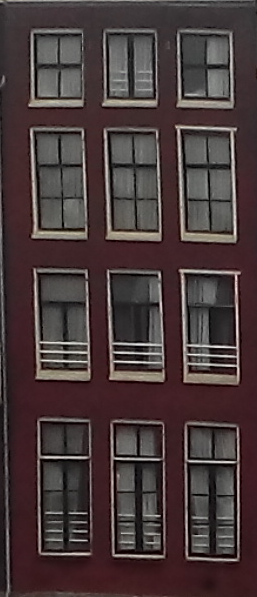
\includegraphics[width=20mm]{bldg.png}
    						\caption{Reality}
						\label{bldg}
  					\end{minipage}
 					 \hfill
					\begin{minipage}[b]{0.4\textwidth}
						\centering
 				  	 	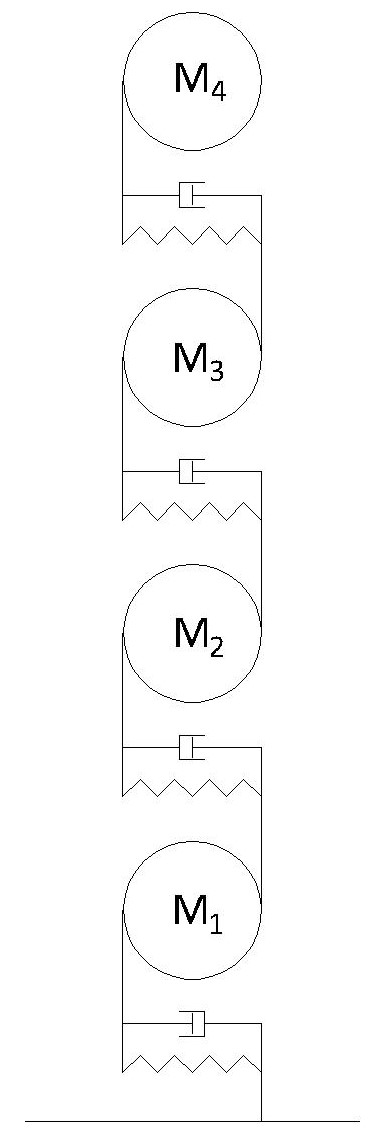
\includegraphics[width=15mm]{SPRINGS-Model1A.jpg}
    						\caption{Simplification}
						\label{Springs1}
 					 \end{minipage}
				\end{figure}

				\item Consider mass $m_i$, spring constant $k_i$, damping constant $c_i$, displacement $x_i$,  and velocity $v_i$of the $i^{th}$ floor
			\end{itemize}
			\bigskip
		\end{frame}
%PHYSICAL DESCRP	%%%%%%%%%%%%%%%%%%%%%%%%%%%%%%%%%%%%%%%%%%%%%%%
		\begin{frame}
  			\frametitle{Physical Description}
			\begin{itemize}
				\item Forces on each floor depend on the floors above and below
				\begin{figure}
 				 	\begin{minipage}[b]{0.4\textwidth}
						\centering
    						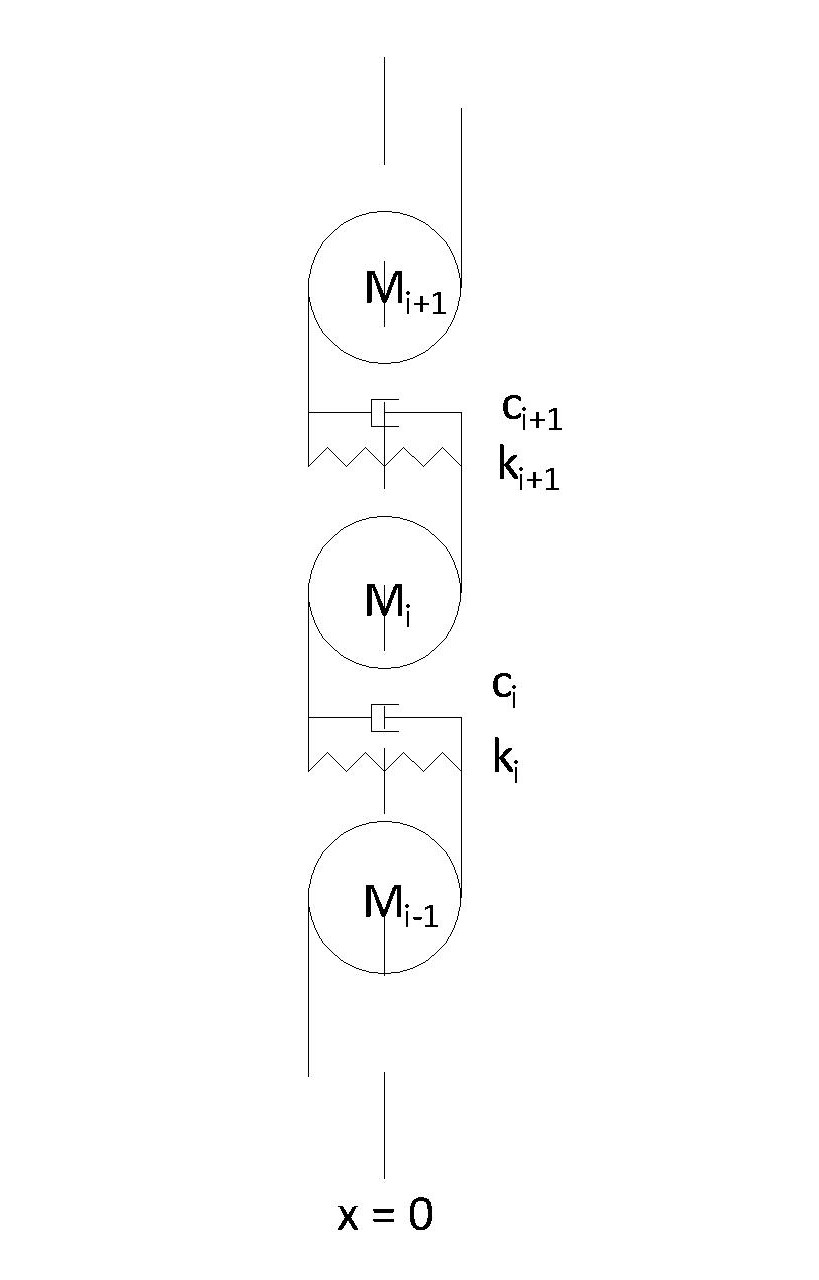
\includegraphics[width=30mm]{SPRINGS-Model2A.jpg}
    						\caption{$i^{th}$ floor statics}
						\label{Springs2}
  					\end{minipage}
 					\hfill
					\begin{minipage}[b]{0.4\textwidth}
						\centering
 				  		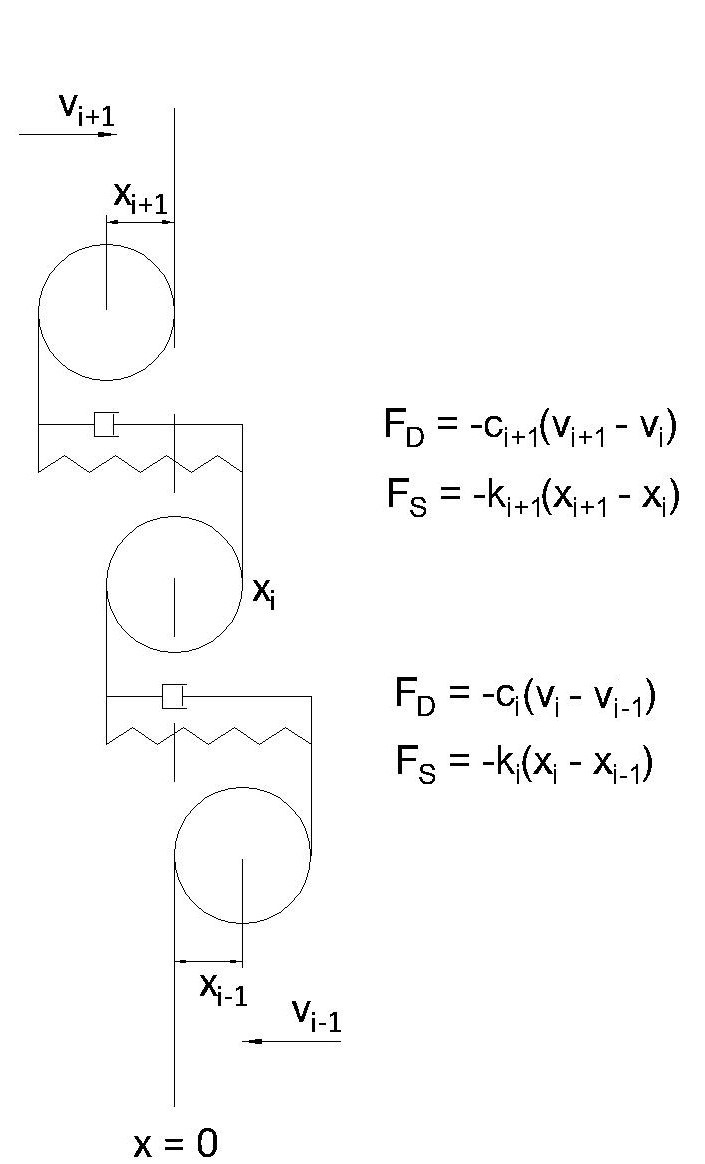
\includegraphics[width=28mm]{SPRINGS-Model3A.jpg}
    						\caption{$i^{th}$ floor dynamics}
						\label{Springs3}
 					\end{minipage}
				\end{figure}
				\item Hooke's law describes the spring force $F_S = - kx$
				\item A linear damping force is considered in a similar manner $F_D = - c\dot{x}$
			\end{itemize}

		\end{frame}
%MOTION EQ	%%%%%%%%%%%%%%%%%%%%%%%%%%%%%%%%%%%%%%%%%%%%%%%%%%
		\begin{frame}
  			\frametitle{Equation of Motion}
			\begin{itemize}
				\item Define matrices for $n$ floors
			\end{itemize}

				\begin{equation*}
					\textbf{K}=
					\begin{bmatrix}
						k_1 + k_2 & -k_2 & 0 & 0 & \cdots & 0 & 0 & 0\\
						-k_2 & k_2 + k_3 & -k_3 & 0 & \cdots & 0 & 0 & 0\\
						\vdots & \vdots & \vdots & \vdots & \ddots & \vdots & \vdots & \vdots \\
						0& 0 & 0 & 0 & \cdots & 0 & -k_{n} & k_{n}\\
					\end{bmatrix},\ \ 
				\end{equation*}\\

				\begin{equation*}
					\textbf{C}=
					\begin{bmatrix}
					           c_1 + c_2 & -c_2 & 0 & 0 & \cdots & 0 & 0 & 0\\
						-c_2 &  c_2 + c_3 & -c_3 & 0 & \cdots & 0 & 0 & 0\\
						\vdots & \vdots & \vdots & \vdots & \ddots & \vdots & \vdots & \vdots \\
						0& 0 & 0 & 0 & \cdots & 0 &-c_{n-1} & c_{n}\\ 
					\end{bmatrix},\ \ 
				\end{equation*}\\

				\begin{equation*}
					\textbf{M}=
					\begin{bmatrix}
						m_1 & 0 & 0 & \cdots & 0\\
						0 & m_2 & 0 & \cdots & 0\\
						\vdots & \vdots & \vdots & \ddots & \vdots \\
						0 & 0 & 0 & \cdots & m_n
					\end{bmatrix},\ \ 
					F=
					\begin{bmatrix}
						f_1(t)\\
						0\\
						\vdots \\
						0
					\end{bmatrix},\ \
					X=
					\begin{bmatrix}
						x_1(t)\\
						\vdots \\
						x_n(t)
					\end{bmatrix}
				\end{equation*}
				\begin{framed}
					\begin{equation}\label{MotionEQ}
						\textbf{M}\ddot{X}+\textbf{C}\dot{X}+\textbf{K}X = F
					\end{equation}
				\end{framed}
		\end{frame}
%NUM SOL	%%%%%%%%%%%%%%%%%%%%%%%%%%%%%%%%%%%%%%%%%%%%%%%%%%%%%
		\begin{frame}
  			\frametitle{Numerical Solution}
			\begin{itemize}
				\item Discrete equation from continuous equation of motion (\ref{MotionEQ})
				\begin{equation}
					\textbf{M}A_{n+1}+\textbf{C}V_{n+1}+\textbf{K}D_{n+1} =F_{n+1}
				\end{equation}
				\item Transformation to first order problem
				\begin{equation}
					W_{n+1}=\textbf{H}U_{n+1} + \textbf{P}
				\end{equation}

				\begin{equation*}
					W_{n+1}=
					\begin{bmatrix}
						V_{n+1}\\ A_{n+1}
					\end{bmatrix}
					\text{,     } U_{n+1}=
					\begin{bmatrix}
						D_{n+1}\\ V_{n+1}
					\end{bmatrix} 
					\text{     ,     }\textbf{H} = 
					\begin{bmatrix} 
						\textbf{0} & \textbf{I} \\ -\textbf{G} &-\textbf{Q} 
					\end{bmatrix}
				\end{equation*} 

				\begin{equation*} 
					\textbf{P} = 
					\begin{bmatrix}
			 			0\\ \textbf{M}^{-1} F_{n+1}
					\end{bmatrix}
					\text{,     }\textbf{G} = \textbf{M}^{-1}\textbf{C}\text{, and            }\textbf{Q} = \textbf{M}^{-1} \textbf{K}\text{.}
				\end{equation*}
				\item Numerical solutions have to behave as the true analytical solution (stability and error in the numerical solution have to be analyzed).
			\end{itemize}
		\end{frame}
%STAB	%%%%%%%%%%%%%%%%%%%%%%%%%%%%%%%%%%%%%%%%%%%%%%%%%%%%%
		\begin{frame}
  			\frametitle{Stability}
			\begin{itemize}
				\item  Stability: resistance of a solution to change; the solution remains within certain bounds and does not grow to infinity.
				\item Amplification matrix $A$ ($n \times n$)
					\begin{equation}
						\dot{U} = \textbf{A}U
						\text{, where } U = 
							\begin{bmatrix}
								X\\\dot{X}
							\end{bmatrix}
					\end{equation} 
				\item Transform system by using the following property (\ref{diag}) and substitution (\ref{sub})
					\begin{equation}\label{diag}
						\textbf{V}^{-1} \textbf{A} \textbf{V}= \textbf{diag} (\lambda_i) = \textbf{ $\Lambda$ }
					\end{equation}
					\begin{equation}\label{sub}
						U = \textbf{V}Y
					\end{equation}
				\item Eigenvalue amplification matrix ($\textbf{$\Lambda$}$ causes amplification if the eigenvalues $> 1$)
					\begin{equation}
						\dot{Y} = \textbf{$\Lambda$ }Y
					\end{equation}	
				\item Here the term $\textbf{$\Lambda$}$ causes amplification if the eigenvalues are greater than 1.
				\item The spectral radius is defined as
					\begin{equation*}
						\rho = \text{max}_i^n(\lambda_i)
					\end{equation*}
				\item The stability conditions to prevent amplification are:
					\begin{itemize}	
						\item $\rho \leq 1$ 
						\item repeated eigenvalues are strictly less than 1
					\end{itemize}
			\end{itemize}
		\end{frame}
%EULER	%%%%%%%%%%%%%%%%%%%%%%%%%%%%%%%%%%%%%%%%%%%%%%%%%%%%%
		\begin{frame}
  			\frametitle{Euler Method}
			\begin{itemize}
				\item Simplest numerical method
				\begin{align}\label{Euler}
					&\text{Backward Euler (implicit):  }U_{n+1} = U_n + h\dot{U}_{n+1}\\
					&\text{Forward Euler (explicit):  }U_{n+1} = U_n + h\dot{U}_{n}
				\end{align} where the time-step $h = t_{n+1}-t_n$
				\item Stability conditions
					\begin{equation}
						 h\rho = 1 - e^{-i\theta}
					\end{equation}
					\begin{equation}
						 h\rho = e^{i\theta} - 1
					\end{equation}
				\begin{figure}
 				 	\begin{minipage}[b]{0.4\textwidth}
						\centering
    						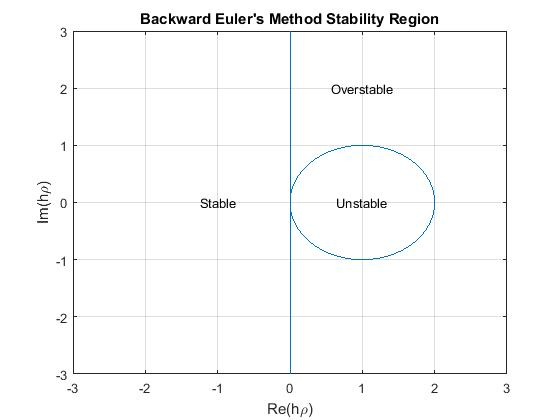
\includegraphics[width=40mm]{GraphEulerB.jpg}
    						\caption{BE stability region}
						\label{Springs2}
  					\end{minipage}
 					\hfill
					\begin{minipage}[b]{0.4\textwidth}
						\centering
 				  		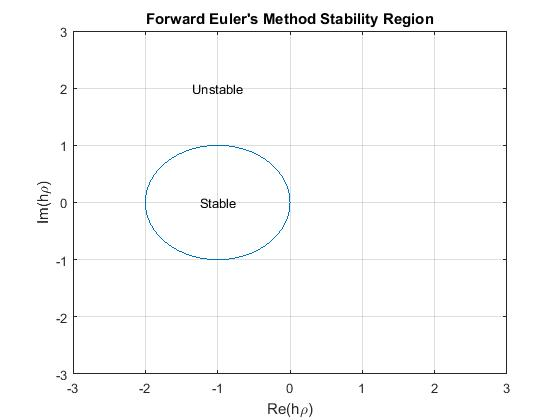
\includegraphics[width=40mm]{GraphEulerF.jpg}
    						\caption{FE stability region}
						\label{Springs3}
 					\end{minipage}
				\end{figure}
			\end{itemize}
		\end{frame}
%NEWMARK		%%%%%%%%%%%%%%%%%%%%%%%%%%%%%%%%%%%%%%%%%%%%%%%%%%
		\begin{frame}
  			\frametitle{Newmark Method}
			\begin{itemize}
				\item Discretization of position and velocity using truncated Taylor series expansions that have defined constants $\beta$ and $\gamma$
				\begin{align}
					&D_{n+1} = D_{n}+V_{n}\Delta t+\frac{A_{{n}}{\Delta t}^{2}}{2}+2\beta \dot{A}_{n}{\Delta t}^3
					&V_{n+1} = V_{n}+A_{n}\Delta t+\gamma \dot{A}_{n} \Delta t^2
				\end{align}
				\item Definition of derivative
				\begin{equation*}
					\dot{A}_{n} = \frac {A_{{n+1}}-A_{{n}}}{\Delta t}
				\end{equation*}
				\item The Newmark method is defined by the following 3 equations
				\begin{equation}
					\textbf{M}A_{n+1}+\textbf{C}V_{n+1}+\textbf{K}X_{n+1} =F_{n+1}
				\end{equation}

				\begin{equation}
					D_{n+1} = D_{n}+V_{n}\Delta t+\frac{{\Delta t}^{2}}{2}[(1-2\beta)A_n + 2\beta A_{n+1}]
				\end{equation}

				\begin{equation}
					V_{n+1} = A_{n}+\Delta t[(1-\gamma)A_n + \gamma A_{n+1}]
				\end{equation}

			\end{itemize}
		\end{frame}
%NEWMARK IMPL		%%%%%%%%%%%%%%%%%%%%%%%%%%%%%%%%%%%%%%%%%%%%%%%
		\begin{frame}
  			\frametitle{Implementation of Newmark Method}
			\begin{enumerate}
				\item Using initial conditions $D_0$ and $V_0$ calculate $A_0$
					\begin{equation*}
						A_{{0}}= \textbf{M}^{-1} (F_{{0}} -\textbf{C}V_{{0}}-\textbf{K}D_{{0}})
					\end{equation*}
				\item Define constants
					\begin{align*}
						&c_1 = {\frac {1}{{\beta \Delta t}^{2}}}\ \ \ \ \ c_2 =\frac{1}{\beta \Delta t }\ \ \ \ \ c_3 = \frac{1}{2\beta}-1\\
						&c_4 = \frac {\gamma}{\beta \Delta t}\ \ \ \ \ c_5 = 1-{\frac {\gamma}{\beta}}\ \ \ \ \ c_6 = \Delta t \left( 1-{\frac {\gamma}{2\beta}} \right)
					\end{align*}
				\item Define inverted matrix allowing for explicit calculation of $d_{n+1}$
					\begin{equation*}
						\textbf{W}=\left[{\frac {\textbf{M}}{{\Delta t}^{2}\beta}}+{\frac {\textbf{C}\gamma}{\Delta t\,\beta}}+\textbf{K}\right]^{-1}
					\end{equation*}
				\item For each time step calculate $D_{n+1}$, $V_{n+1}$ and $A_{n+1}$
					\begin{align*}
						&\widetilde{A}_{{n+1}}=-c_1D_n+c_2V_n+c_3A_n\\
						&\widetilde{V}_{{n+1}}=c_4D_n+c_5V_n+c_6A_n\\
						&D_{{n+1}}=\textbf{W}[F_{{n+1}}+\textbf{M}\widetilde{A}_{{n+1}}-\textbf{C}\widetilde{V}_{{n+1}}]
					\end{align*}
			\end{enumerate}
		\end{frame}
%NEWMARK STAB1		%%%%%%%%%%%%%%%%%%%%%%%%%%%%%%%%%%%%%%%%%%%%%%%
		\begin{frame}
  			\frametitle{Stability of Newmark Method}
			\begin{itemize}
				\item Writen in first-order form the Newmark method amplification matrix becomes
				\begin{equation}
					U_{n+1} = \textbf{A}U_n
				\end{equation}
where 

				\begin{equation}
					\textbf{A} = \textbf{A}_1^{-1}\textbf{A}_2
				\end{equation}

				\begin{equation}
					\textbf{A}_1 = \begin{bmatrix} \textbf{M}+ \textbf{K} \beta \Delta t^2 & \textbf{C} \beta \Delta t^2 \\
\textbf{K} \gamma \Delta t & \textbf{M} + \textbf{C}\gamma \Delta t\end{bmatrix} 
				\end{equation}

				\begin{equation}
					\textbf{A}_2 = 
						\begin{bmatrix} 
						\textbf{M}- \textbf{K}(1 - 2\beta)\frac{\Delta t^2}{2} & \textbf{M} \Delta t -  \textbf{C}(1 - 2\beta)\frac{\Delta t^2}{2} \\
						\textbf{K}(\gamma - 1)\Delta t & \textbf{M} - \textbf{C}(1 - \gamma)\Delta t
						\end{bmatrix}
				\end{equation}
			\end{itemize}
		\end{frame}
%NEWMARK SATB2	%%%%%%%%%%%%%%%%%%%%%%%%%%%%%%%%%%%%%%%%%%%%%%%%
		\begin{frame}
  			\frametitle{Undamped motion}
			\begin{itemize}
				\item Uncoupled equations of motion
				\begin{align}
				&a_n + \omega^2 d_n = \phi_n\\
				&a_{n+1} + \omega^2 d_{n+1} = \phi_{n+1}
				\end{align}
				\item Characteristic equation
					\begin{equation}
						\lambda^2 - \lambda \left[2 - (\gamma + \frac{1}{2})\epsilon^2\right] + 1 - (\gamma - \frac{1}{2})\epsilon^2 =0
					\end{equation}
				\item Introduce
				$\Omega = \Delta t \omega$ and $T = 1+\beta \Omega^2$. Let $\epsilon^2 = \frac{\Omega^2}{T}$.
			\end{itemize}
%NEWMARK ACC		%%%%%%%%%%%%%%%%%%%%%%%%%%%%%%%%%%%%%%%%%%%%%%%
		\begin{frame}
  			\frametitle{Accuracy of Newmark Mehthod}
			\begin{itemize}
				\item fkj
			\end{itemize}
		\end{frame}
%SIMPLE EXAMPLE		%%%%%%%%%%%%%%%%%%%%%%%%%%%%%%%%%%%%%%%%%%%%%%%
		\begin{frame}
  			\frametitle{Simple example}
			\begin{itemize}
				\item fkj
			\end{itemize}
		\end{frame}
%EL CENTRO	%%%%%%%%%%%%%%%%%%%%%%%%%%%%%%%%%%%%%%%%%%%%%%%%%%
		\begin{frame}
  			\frametitle{El Centro earthquake}
			\begin{itemize}
				\item fkj
			\end{itemize}
		\end{frame}
%14	%%%%%%%%%%%%%%%%%%%%%%%%%%%%%%%%%%%%%%%%%%%%%%%%%%%%%%%%
		\begin{frame}
  			\frametitle{}
		\end{frame}
%15	%%%%%%%%%%%%%%%%%%%%%%%%%%%%%%%%%%%%%%%%%%%%%%%%%%%%%%%%
		\begin{frame}
  			\frametitle{}
		\end{frame}
%%%%%%%%%%%%%%%%%%%%%%%%%%%%%%%%%%%%%%%%%%%%%%%%%%%%%%%%%%%
\end{document}